% Chapter 5 text
\chapter{Hydrologic controls on the seasonal and inter-annual variability in Congo River particulate organic carbon sources and reservoir age}
\label{Ch5}
\raggedbottom

{\let\thefootnote\relax\footnotetext{This chapter is currently in preparation for submission as: Hemingway J.D., Schefu\ss \ E., Spencer R.G.M., Dinga B.J., Eglinton T.I., McIntyre C., and Galy V.V. {Hydrologic controls on the seasonal and inter-annual variability in Congo River particulate organic carbon and GDGT sources.}}}

\clearpage

\section{Abstract}

Tropical rivers are a major source of organic matter (OM) to the coastal ocean and play a large role in the global carbon cycle. As such, it is critical to understand the sources, sinks, and transformations of OM during fluvial transit over seasonal and inter-annual timescales. Here we present dissolved organic carbon (DOC) concentrations, particulate OM (POM) composition (\ce{\delta^{13}C}, \ce{\delta^{15}N}, \ce{\Delta^{14}C}, N/C), and glycerol dialkyl glycerol tetraether (GDGT) biomarker distributions from a 34-month time-series near the mouth of the Congo River.

An end-member mixing model based on \ce{\delta^{13}C} and N/C indicates that exported POM is consistently dominated by C\textsubscript{3} tropical rainforest soil inputs, with increasing contributions by C\textsubscript{3} tropical plant vegetation and decreasing contributions by autochthonous phytoplankton at high discharge. Inputs from C\textsubscript{4} plants and soils are negligible throughout the time-series despite covering $\approx 13$\% of the catchment. Calculated \ce{\Delta^{14}C} values of the C\textsubscript{3}-soil end member reveal significant and variable pre-aging prior to export, especially during the year 2011 when southern-hemisphere discharge reached record lows (mean = $-176$\textperthousand, standard deviation = $93$\textperthousand). In contrast, soil \ce{\Delta^{14}C} values were stable near $-50$\textperthousand\ between January and June 2013 when southern-hemisphere discharge was highest. These results indicate that headwater POM is diluted and/or overprinted by C\textsubscript{3} vegetation and pre-aged soils during transit through the \textit{Cuvette Congolaise} swamp forest, while left-bank tributaries export significantly less pre-aged material.

Glycerol dialkyl glycerol tetraether (GDGT) biomarker distributions provide further evidence for changes in soil provenance, as branched and isoprenoid GDGT distributions both exhibit large seasonal and inter-annual variability. Methylation and cyclization of branched tetraethers (MBT', CBT) and the GDGT-0/crenarchaeol ratio (GDGT-0/cren) are positively correlated with discharge ($r \geq 0.62$; $p$-value $\leq 1.39 \times 10^{-4}$) and reflect a significant incorporation of compounds produced in permanently inundated \textit{Cuvette Congolaise} swamp-forest soils, especially in 2011, thus highlighting the importance of this region in controlling organic carbon export.

\section{Introduction}

River networks act as a dynamic link between terrestrial and aquatic ecosystems and play a major role in the global carbon cycle via the weathering of silicate minerals \citep{Berner:1983uk,Gaillardet:1999uy}, oxidation of rock-derived organic carbon \citep[OC\textsubscript{petro};][]{Galy:2008ff,Bouchez:2010if,Hilton:2014dh}, and export of biospheric particulate OC (POC) to the coastal ocean coupled with subsequent burial in marine sediments \citep{Berner:1982vg,Galy:2007ev}. Additionally, because POC buried in large fluvial fans is typically thought to integrate over a wide geographic area, paleo-environmental proxies such as bulk \ce{\delta^{13}C}, plant-wax \ce{\delta^{13}C}, and glycerol dialkyl glycerol tetraether (GDGT) molecular distributions in sedimentary archives are commonly used to reconstruct past ecosystem coverage and environmental conditions \citep[\textit{e.g.}][]{FranceLanord:1994vp,Freeman:2001tv,Schefuss:2005jo,Weijers:2007fp}.

There has thus been a significant effort to determine the geologic and climatic controls on the source, composition, and export flux of biospheric POC in modern rivers across the globe due to the fact that burial of this material in marine sediments constitutes a net atmospheric \ce{CO2} sink \citep{Lasaga:1985ts,Ludwig:1996ul,Galy:2015fx}. Furthermore, it is now known that rivers are generally not passive conduits to the ocean, but rather integrate, process, and remineralize multiple sources of terrestrial (allochthonous) and aquatic (autochthonous) organic matter (OM) during transit \citep{Cole:2007gp,Aufdenkampe:2011fm}. For example, \citet{Galy:2008jw,Galy:2011ix} analyzed the \ce{^{13}C} composition of bulk POC and plant-wax \textit{n}-alkanoic acids in Ganges-Brahmaputra suspended sediments to conclude that headwater Himalayan C\textsubscript{3} material is replaced by a floodplain-derived mixed C\textsubscript{3}/C\textsubscript{4} signal prior to export. Similarly, downstream decreases in bulk \ce{^{13}C} composition and carbon-normalized lignin concentration have been observed in Amazon River fine-grained POC and are attributed to the addition of floodplain soil material \citep{Hedges:1986ab,Hedges:2000tn}.

Specific to the Congo Basin, recent studies based on the isotope composition of dissolved lithium and silicon suggest that "black water" rivers such as those draining the permanently inundated \textit{Cuvette Congolaise} swamp forest (Figure \ref{Ch5Fig:1}A) contribute $\approx 30$\% of the water discharged at Brazzaville/Kinshasa annually, with significantly higher contributions during peak discharge \citep{Cardinal:2010ir,Henchiri:2016jh}. However, the mechanisms controlling the influence of this end member on exported suspended sediments in general and particulate OM (POM) in particular remain unknown \citep{Spencer:2016ho}.

% Figure 1
\begin{figure}[ht]
	\makebox[\textwidth][c]{\includegraphics[]{Thesis_Figures/Ch5Fig1}}
	\caption[Congo catchment map showing landcover and \%C\textsubscript{3} vs. \%C\textsubscript{4} vegatation]{Congo, Djoue, and Oubangui catchment outlines showing $(A)$ ecosystem landcover \citep{Mayaux:2004uw} and $(B)$ C\textsubscript{3}/C\textsubscript{4} landcover \citep{Still:2010wh}. Our sampling location is marked as a red circle (this marker covers both the Congo and Djoue River sampling sites), while Bangui Station \citep{Bouillon:2012cw,Bouillon:2014ko} is marked as a white diamond. Djoue and Oubangui River sub-basins upstream of each sampling location are highlighted in pastel colors.}
	\label{Ch5Fig:1} 
\end{figure}

Still, \citet{Laraque:2009fz} observe a decrease in sediment yield downstream of the \textit{Cuvette Congolaise} as compared to upstream tributaries, suggesting that a significant amount of headwater material can settle out during passage through this central depression. Exported sediments are therefore biased downstream, as evidenced by the \ce{^{13}C} and molecular composition of exported plant-wax \textit{n}-alcohols and \textit{n}-alkanoic acids, which are consistently dominated by a swamp-forest-derived C\textsubscript{3} signal during periods of high discharge \citep{Hemingway:2016bq}. Furthermore, millennial-scale changes in climate and hydrology likely influence the ability of the \textit{Cuvette Congolaise} to act as an OM reservoir and POM source. For example, \citet{Schefuss:2016cp} show that the terrestrial reservoir age of exported plant waxes has been steadily increasing since the humid Early- to Mid-Holocene ($\approx$10,000--5,000 years before present), suggesting that pre-aged \textit{Cuvette}-derived OM is remobilized during periods of decreased rainfall in the basin.

Despite these findings, quantitatively partitioning POM sources and understanding the mechanisms that control their variability on seasonal and inter-annual timescales remains an open question in the Congo River system. To estimate POM source contributions, multiple (pseudo-)conservative tracers such as \ce{\delta^{13}C}, \ce{\Delta^{14}C}, and the N/C ratio are frequently used in end-member mixing models \citep{Perdue:2007fn,Weijers:2009iu,Hilton:2010cg,Hossler:2012jh}, although this requires that end-member compositions are well-constrained and can lead to spurious results if temporal variability in such composition is unknown. Still, this method has been successfully utilized to separate OM sources in riverine suspended sediments \citep{Hilton:2010cg,Hossler:2012jh} and to calculate terrestrial contribution to continental shelf sediments \citep{Gordon:2004id,Weijers:2009iu}. 

In addition to bulk measurements, microbial GDGT membrane lipids can offer further insight as a tracer for OM sources. The concentrations and molecular compositions of both branched (brGDGTs) and isoprenoid (isoGDGTs) GDGTs have become a commonly used proxy to determine the source of POM in a host of environments and to record environmental conditions such as temperature and soil pH \citep[see][for review]{Castaneda:2011jb,Schouten:2013bd}. For example, because brGDGTs are thought to be produced predominantly in soils while isoGDGTs are dominant in aquatic environments, the branched to isoprenoid tetraether (BIT) index first described by \citet{Hopmans:2004kx} is often used in fluvial suspended sediments \citep{Kim:2012fq,Zell:2014gt}, lacustrine sediments \citep{Tierney:2010br}, and continental shelf sediments \citep{Peterse:2009hl,Weijers:2009iu} to estimate soil OM contribution. Furthermore, the methylation of branched tetraether (MBT') and cyclization of branched tetraether (CBT) indices have been shown to co-vary with temperature and pH in a global soil dataset \citep{Weijers:2007gu,Peterse:2012bs,DeJonge:2014kw} and have thus been utilized in large fluvial catchments as a tracer of OC source \citep{Zell:2013eg,DeJonge:2014fs}. Because the Congo River covers multiple ecosystems that are described by a range of environmental conditions such as soil pH \citep{Mayaux:2004uw,Spencer:2012en}, GDGT signals should provide an additional constraint on exported POM provenance.

Combined, bulk POM and GDGT temporal and spatial variability imply that POM and biomarker geographic integration in large river systems is non-uniform and that exported signals are likely subject to large seasonal/inter-annual changes in end-member contribution \citep[\textit{e.g.}][]{Galy:2008jw,Zell:2013eg,Spencer:2016ho}. To understand this variability in the Congo basin, we extend published records of Congo River main-stem OM \citep{Mariotti:1991vx,Coynel:2005cn,Spencer:2012en,Hemingway:2016bq,Spencer:2016ho} by reporting dissolved organic carbon (DOC) concentrations, POM composition (\ce{\delta^{13}C}, \ce{\delta^{15}N}, \ce{\Delta^{14}C}, N/C), and GDGT distributions from a 34-month time-series collected at Brazzaville/Kinshasa (see Table \ref{Ch5Tab:1}; Figure \ref{Ch5Fig:1} for sampling locations). Additionally, we present bulk POM measurements (\ce{\delta^{13}C}, \ce{\delta^{15}N}, N/C) from the Djoue River, a small mixed C\textsubscript{3}/C\textsubscript{4} end-member tributary near Brazzaville, for a 13-month subset of this time-series. Combined with a previously published 2-year time-series from the Oubangui River upstream of the \textit{Cuvette Congolaise}  \citep{Bouillon:2012cw,Bouillon:2014ko}, our results thus provide an understanding of POM source evolution during fluvial transit through this permanently inundated swamp forest. Lastly, we discuss the influence of climate and hydrology on the \textit{Cuvette Congolaise} as a POM source both on inter-annual timescales and with respect to paleo-environmental records derived from the Congo Fan.

% Table 1
\begin{table}[ht]
	\caption[Congo, Djoue, and Oubangui catchment properties and landcover composition]{Congo, Djoue, and Oubangui catchment properties and landcover composition.}
	\makebox[\textwidth][c]{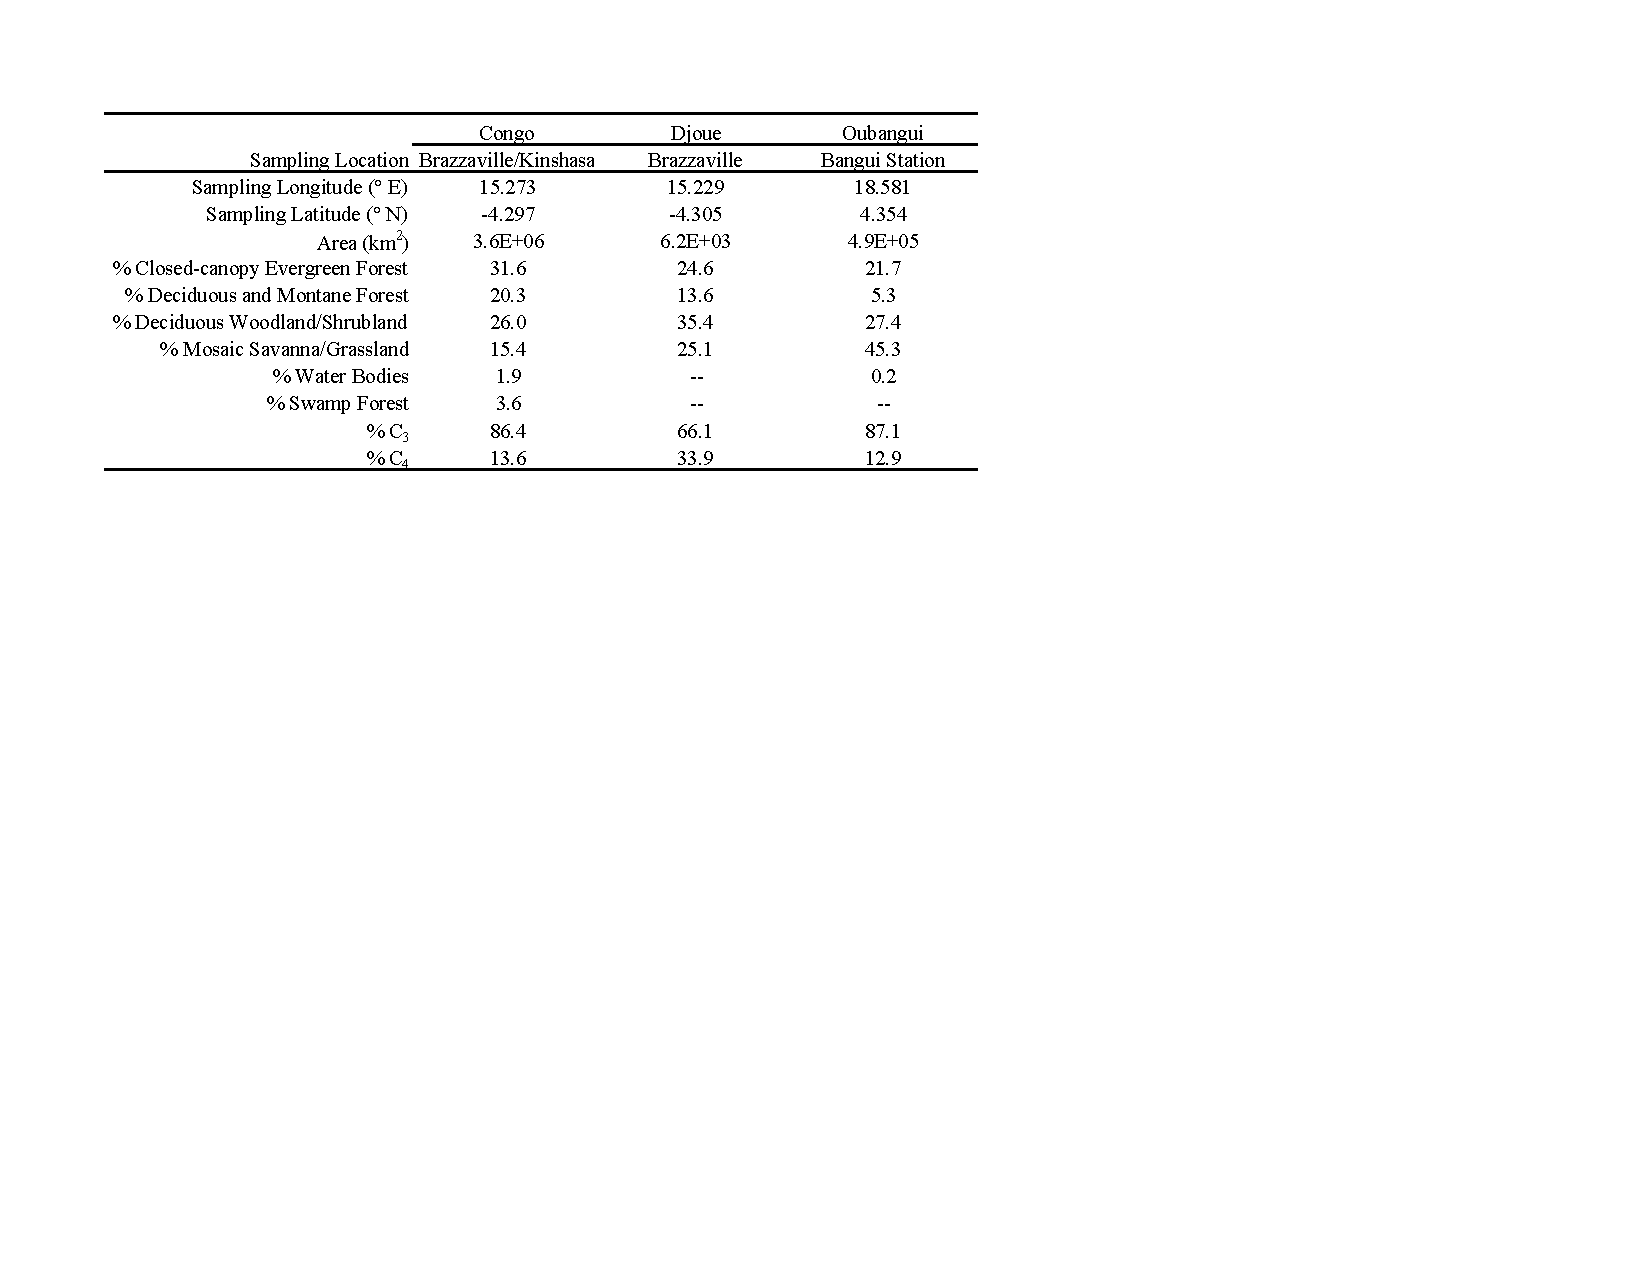
\includegraphics[]{Thesis_Tables/Ch5Tab1}}
	\label{Ch5Tab:1} 
\end{table}

\section{Study Site}

The Congo River drains $3.6 \times 10^6$ km\textsuperscript{2} of central Africa between $10$\textdegree N and $15$\textdegree S and is highly influenced by the seasonal north-to-south migration of the inter-tropical convergence zone \citep[ITCZ;][]{Gasse:2000ul}. This leads to strong latitudinal gradients in vegetation and ecosystem type \citep{Mayaux:2004uw}, including the \textit{Cuvette Congolaise} swamp forest (Figure \ref{Ch5Fig:1}A), and corresponding changes in C\textsubscript{3} vs. C\textsubscript{4} landcover \citep[Figure \ref{Ch5Fig:1}B;][]{Still:2010wh}. The Congo basin is dominated by closed-canopy evergreen forest near the equator and deciduous woodland/shrubland at the northern and southern peripheries, with smaller contributions by deciduous and montane forests, mosaic savanna/grassland, and swamp forest (Table \ref{Ch5Tab:1}). In contrast, both the Oubangui sub-basin upstream of Bangui Station and the Djoue River contain mostly mosaic savannah/grassland and deciduous woodland/shrubland. This leads to $\geq 85$\% C\textsubscript{3} landcover in the Congo and Oubangui basins, while the Djoue exhibits more evenly mixed C\textsubscript{3}/C\textsubscript{4} coverage (Table \ref{Ch5Tab:1}).

Congo River discharge (Q\textsubscript{w}) recorded at Brazzaville/Kinshasa is remarkably stable and predictable, with an annual maximum near $50,000$ m\textsuperscript{3} s\textsuperscript{-1} and a minimum near $25,000$ m\textsuperscript{3} s\textsuperscript{-1} \citep[Figure \ref{Ch5Fig:2}A;][]{Coynel:2005cn,Laraque:2009fz,Spencer:2014vp}. Increased precipitation in the north of the catchment between May and September \citep{Mahe:1993wu} and a $\approx 1 - 2$ month transit time \citep{Bricquet:1993ve} leads to discharge maxima of right-bank (\textit{i.e.} northern-hemisphere) tributaries such as the Oubangui River during Nov-Dec-Jan \citep{Coynel:2005cn,Bouillon:2012cw,Bouillon:2014ko} and corresponds to elevated water flux through the \textit{Cuvette Congolaise} during this time. Between November and March, southern-hemisphere precipitation increases left-bank tributary contribution in response to the seasonal ITCZ migration and is the source of the secondary discharge maximum observed during Apr-May-Jun \citep[Figure \ref{Ch5Fig:2}A;][]{Bricquet:1993ve,Mahe:1993wu}. Importantly, the largest left-bank tributary (Kasai River) enters the main-stem downstream of the \textit{Cuvette Congolaise}. In contrast to the Congo River main-stem, Oubangui River discharge is highly seasonal, ranging from $\approx 300$ m\textsuperscript{3} s\textsuperscript{-1} in Mar-Apr-May to $\approx 9,000$ m\textsuperscript{3} s\textsuperscript{-1} in Oct-Nov-Dec \citep{Bouillon:2012cw,Bouillon:2014ko}.

% Figure 2
\begin{figure}[p]
	\makebox[\textwidth][c]{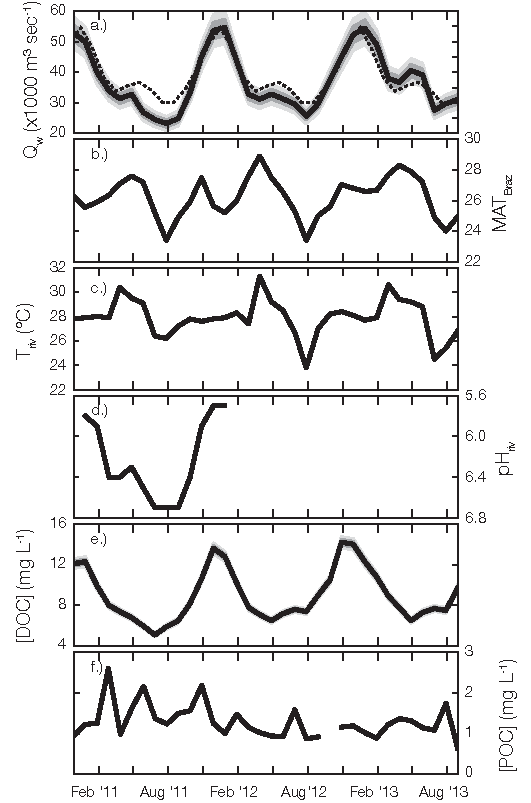
\includegraphics[]{Thesis_Figures/Ch5Fig2}}
	\caption[Environmental parameter time-series plots]{Time-series plots of Congo River $(A)$ discharge (Q\textsubscript{w}), $(B)$ mean monthly air temperature at Brazzaville/Kinshasa (MAT\textsubscript{Braz}), $(C)$ measured river water temperature (T\textsubscript{riv}), $(D)$ measured river water pH from \citet{Wang:2013js} (pH\textsubscript{riv}), $(E)$ DOC concentration ([DOC]), and $(F)$ POC concentration ([POC]) from \citet{Hemingway:2016bq}. Where visible, dark gray envelope is $\pm 1 \sigma$ uncertainty and light gray envelope is 95\% confidence interval. Dotted line in panel $(A)$ is the 1977--2006 (inclusive) average hydrograph \citep{Spencer:2012en}.}
	\label{Ch5Fig:2} 
\end{figure}

\section{Materials and Methods}

\subsection{Sample collection}

Congo River samples were collected monthly between November 2010 and August 2013 near Brazzaville/Kinshasa, just downstream of the Pool Malebo and $\approx 300$ km upstream of the Congo Estuary (Table \ref{Ch5Tab:1}; Figure \ref{Ch5Fig:1}), while Djoue River samples were similarly collected between November 2010 and November 2011. The Congo River sampling location is downstream of all major tributaries, capturing $>95$\% of the total catchment \citep{Spencer:2012en}. Water for total suspended sediments (TSS) was collected from the surface of the river and filtered through $0.22 \mu$m polyether sulfone (PES) membrane filters. After drying ($60$\textdegree C) and shipment, samples were re-suspended in $18$M$\Omega$ Milli-Q water, freeze-dried, and weighed for TSS concentration. Simultaneously, Congo River water was collected for DOC analysis and filtered through $0.7 \mu$m pre-combusted ($550$\textdegree C, 4 hours) GF/F filters into acid pre-leached and triple sample-rinsed HDPE bottles. DOC samples were acidified to pH $2$ using trace-metal grade HCl and immediately frozen until further analysis.

Surface water temperatures (T\textsubscript{riv}) were measured concurrently using a YSI Professional Plus multiparameter instrument (YSI Incorporated) and daily Congo River discharge was measured at a nearby gauging station operated by the Institute de Recherche en Sciences Exactes et Naturelles (Republic of Congo) using a rating curve that is periodically updated by Acoustic Doppler Current Profiler (ADCP) transects. Triplicate ADCP transects suggest that river discharge measurements are precise to $\pm 5$\%, although precision is likely lower during high discharge due to overbank flooding \citep{Spencer:2014vp}. Monthly mean air temperature recorded at Brazzaville/Kinshasa (MAT\textsubscript{Braz}; $4.25$\textdegree S, $15.25$\textdegree E) was obtained from the National Oceanic and Atmospheric Administration (NOAA) National Climate Data Center database. MAT was missing for one month (April 2012) and was therefore estimated as the average between mean daily maximum and minimum temperatures during that month. 

\subsection{Bulk measurements}

DOC concentration ([DOC]) was quantified via high-temperature combustion using a Shimadzu TOC-V organic carbon analyzer. Each sample was injected until there existed triplicate measurements with a coefficient of variability $\leq 2$\%, and was calibrated to a six-point calibration curve after accounting for instrument drift using an internal control standard following \citet{Mann:2012kp}. [DOC] is taken as the mean of these triplicate values with a relative uncertainty ($\pm 1 \sigma$) of $\pm 2$\%.

Organic carbon and nitrogen percentages (\%OC, \%N\textsubscript{org}) and stable isotopes (\ce{\delta^{13}C}, \ce{\delta^{15}N}) were measured on TSS aliquots following the methods of \citet{Whiteside:2011jea}. We note that one sample (September 2012) became contaminated by dissolution of the PES membrane during re-suspension and was therefore omitted from bulk measurements. All other samples were acidified under HCl fumes at $60$\textdegree C for 72 hours to remove carbonates prior to \%OC and \ce{\delta^{13}C} measurement using a Fisons elemental analyzer coupled to a Finnigan Delta\textsuperscript{plus} isotope-ratio mass spectrometer (IRMS). \%N\textsubscript{org} and \ce{\delta^{15}N} measurements were performed similarly but using non-acidified aliquots. All samples were injected in triplicate and calibrated against \ce{CO2} or \ce{N2} gas with known isotope composition. Uncertainty is taken as the standard deviation of triplicate measurements and isotope values are reported as per-mille (\textperthousand) deviations from Vienna Pee Dee Belemnite (VPDB) for \ce{\delta^{13}C} and atmospheric \ce{N2} (AIR) for \ce{\delta^{15}N}.

Aliquots for radiocarbon analysis, along with corresponding process blanks and standards, were subjected to the acidification treatment described above and were oxidized to \ce{CO2} by baking ($850$\textdegree C, 5 hours) with $\approx 1$ g cupric oxide in evacuated and flame-sealed quartz tubes. \ce{CO2} gas was then distilled cryogenically, transferred to Pyrex tubes, and analyzed for radiocarbon content using a mini carbon dating system (MICADAS) accelerator mass spectrometer fitted with a gas-ion source (Ionplus AG) at the Laboratory for Ion Beam Physics, ETH Zurich \citep{Christl:2013ks}. Data are corrected for process blanks and reported following the \ce{\Delta^{14}C} per-mille notation of \citet{Stuiver:1977uh}.

\subsection{GDGT extraction and purification}

Remaining Congo River TSS was extracted at $100$\textdegree C for 20 minutes in a microwave accelerated reaction system (MARS, CEM Corporation) in $20$ mL of dichloromethane (DCM) and methanol (9:1). Because \textit{n}-alkyl lipid isotopes were also measured on these samples \citep{Hemingway:2016bq}, total lipid extracts were saponified at $70$\textdegree C for 2 hours using $0.5$ M KOH in methanol. GDGT distributions reported here therefore represent a combination of core lipids and intact polar phospholipids, as base hydrolysis is known to cleave phosphate-bound head groups \citep{Weijers:2011bn}.

Subsequently, $15$ mL of $18$M$\Omega$ Milli-Q water was added and "base" fractions were liquid-liquid extracted into $5$ mL hexane 5 times. HCl was then added drop-wise until pH $2$ was reached, and "acid" fractions were extracted using 5mL hexane and DCM (4:1) until the organic phase was clear (typically 5 times). Acid and base fractions were separated by column chromatography using $1$ g of Supelclean amino-propyl silica gel (Supelco Analytical) and the following elution scheme: $4$ mL hexane (F1); $7$ mL hexane and DCM (4:1, F2); $10$ mL DCM and acetone (9:1, F3); $14$ mL 2\% (w/w) formic acid in DCM (F4); $18$ mL DCM and methanol (1:1, F5). Acid and base fractions containing GDGTs (F3) were recombined to ensure maximum recovery. To remove \textit{n}-alcohols, combined F3s were subjected to urea adduction in which $500 \mu$L of urea-saturated methanol was added and solvent was evaporated using a stream of \ce{N2} gas to promote urea recrystallization (repeated three times). Crystals were rinsed three times with $5$ mL hexane to remove the "non adducted" fraction containing GDGTs, which was then stored at $4$\textdegree C until analysis. While the additional handling steps described here likely lower GDGT recovery, results from a recent inter-comparison exercise \citep{Schouten:2013hh} indicate that our purification protocol does not impart a significant bias in GDGT distributions as compared to other commonly used methods \citep[\textit{e.g.} the modified Bligh and Dyer method of][]{Pitcher:2009jd}.

\subsection{GDGT detection and analysis}

GDGTs were detected on an Agilent 1200 series high-pressure liquid chromatograph coupled to an Agilent LC/MSD SL quadrupole mass spectrometer (HPLC-MS) as initially described by \citet{Hopmans:2000ti}. Compounds were ionized using atmospheric-pressure chemical ionization (APCI) and detected on their [M+H]\textsuperscript{+} ions in selected ion monitoring (SIM) mode. Chromatographic separation was achieved in normal phase through a Grace Prevail Cyano $3 \mu$m column ($150$ mm $\times$ $2.1$ mm). Samples were injected ($5 \mu$L) and solvent A (99:1 [v/v] hexane:isopropanol) was pumped at $0.2$ mL/min isocratically for 5 minutes, then with a linear gradient for 40 minutes, reaching 10\% solvent B (9:1 [v/v] hexane:isopropanol). We note that this chromatographic method cannot separate multiple co-eluting compounds such as the six distinct peaks at $1050$ m/z observed by \citet{Becker:2013jw} and the recently discovered 6-methyl brGDGTs IIa'--IIIc' \citep[see Figure \ref{Ch5Fig:S1} for structures;][]{DeJonge:2013cr,DeJonge:2014kw}. Such co-elution could potentially alter calculated brGDGT metrics, although this effect is likely negligible in our sample set (see Supplemental Discussion \ref{Ch5SD1}).

A laboratory working standard was injected at multiple concentrations between every 5--10 samples ($n = 32$) and showed $<10$\% variability for all metrics over all concentrations throughout the analysis, indicating minimal instrument drift. Metrics and ratios were calculated based on raw areas (\textit{i.e.} molar ratios), assuming an identical response factor of all isoGDGTs and brGDGTs in accordance with current best practice \citep{Schouten:2013hh,Schouten:2013bd}. Metrics were calculated following the equations of \citet{Hopmans:2004kx}, \citet{Peterse:2012bs}, and \citet{Weijers:2007gu}, respectively:

% Equation 1
\begin{equation}\label{Ch5Eq:1}
	\text{BIT} = \frac{\{\text{brIa}\} + \{\text{brIIa}\} + \{\text{brIIIa}\}}{\{\text{brIa}\} + \{\text{brIIa}\} + \{\text{brIIIa}\} + \{\text{cren}\}}
\end{equation}

% Equation 2
\begin{equation}\label{Ch5Eq:2}
	\text{MBT'} = \frac{\{\text{brIa}\} + \{\text{brIb}\} + \{\text{brIc}\}}{\{\text{brIa}\} + \{\text{brIb}\} + \{\text{brIc}\} + \{\text{brIIa}\} + \{\text{brIIb}\} + \{\text{brIIc}\} + \{\text{brIIIa}\}}
\end{equation}

% Equation 3
\begin{equation}\label{Ch5Eq:3}
	\text{CBT} = -\log \frac{\{\text{brIb}\} + \{\text{brIb}\}}{\{\text{brIa}\} + \{\text{brIIa}\}}
\end{equation}

where $\{j\}$ is the area of the [M+H]\textsuperscript{+} ion for compound $j$, noting that $\{\text{brIIa}\} - \{\text{brIIIa}\}$ represent the sum of co-eluting 5-methyl and 6-methyl compounds \citep{DeJonge:2014kw}. Additionally, the GDGT-0/cren was calculated as $\{\text{GDGT-0}\}/\{\text{cren}\}$ following \citet{Blaga:2009ge}. All samples were injected in triplicate and metrics are reported as the mean and standard deviation of triplicate measurements.

\subsection{Data analysis and model setup}

All regressions were performed as ordinary least squares (OLS) and statistical results are reported as regression coefficients ($r$) and significance $p$-values. Time-series average values are reported as the mean $\pm 1$ standard deviation about the mean. All data analysis was performed in the Python programming language v.2.7 and ArcGIS for Desktop v.10.3.

Quantitative contribution of $m$ end members to bulk POM was determined following optimum multi-parameter analysis (OMPA) using $m-1$ (pseudo-)conservative tracers, as described in \citet{Glover:2011uh}. End-member composition uncertainty was incorporated by \textit{(i)} including a weighting factor for each tracer equal to the range of observed values divided by the average end-member uncertainty and \textit{(ii)} allowing for 1\% deviation in the constraint that fractional contributions sum to unity \citep{Glover:2011uh}. Additionally, because phytoplankton \ce{\delta^{13}C} is known to vary seasonally in the Congo basin \citep{Bouillon:2014ko}, the composition of this end member was allowed to vary and the model was re-initialized for each sample.

To determine the environmental controls on GDGT metrics, redundancy analysis (RDA) was performed following \citet{Legendre:1998tt}. In the resulting triplot, the "site" and "species" scores were scaled symmetrically by the square root of corresponding eigenvalues ("Type III" scaling).

\section{Results}

All environmental parameters and bulk measurements are reported in Table \ref{Ch5Tab:S1} while all GDGT fractional abundances and calculated metrics are reported in Table \ref{Ch5Tab:S2}. 

\subsection{Environmental parameters}

Congo River discharge recorded at Brazzaville/Kinshasa during the time-series ranged from $(23.2 \pm 1.1) \times 10^3$ m\textsuperscript{3} s\textsuperscript{-1} in July 2011 to $(54.6 \pm 2.7) \times 10^3$ m\textsuperscript{3} s\textsuperscript{-1} in December 2011 (Figure \ref{Ch5Fig:2}A). Annual averaged discharge for 2012 and 2013 is near the long-term mean value of $38.8 \times 10^3$ m\textsuperscript{3} s\textsuperscript{-1} (1977--2006 inclusive), however average discharge for 2011 ($35.3 \times 10^3$ m\textsuperscript{3} s\textsuperscript{-1}) is the fifth-lowest in this record \citep{Spencer:2012en}. Importantly, this is due to a significantly suppressed left-bank discharge maximum during Apr-May-Jun as compared to the 1977--2006 mean for these months. In contrast, northern-hemisphere peak discharge (Nov-Dec-Jan) is near the long-term average for all years in the time-series presented here (Figure \ref{Ch5Fig:2}A).

MAT\textsubscript{Braz} correlates strongly with T\textsubscript{riv} (Table \ref{Ch5Tab:2}) and both are relatively invariable over the time-series (Figure \ref{Ch5Fig:2}B, \ref{Ch5Fig:2}C). T\textsubscript{riv} ranges from a minimum of $23.8$\textdegree C to a maximum of $31.3$\textdegree C (mean = $27.9 \pm 1.6$\textdegree C), while MAT\textsubscript{Braz} exhibits similar values, ranging from $23.4$\textdegree C to $28.9$\textdegree C (mean = $26.2 \pm 1.3$\textdegree C). Both T\textsubscript{riv} and MAT\textsubscript{Braz} are uncorrelated with all other environmental parameters, bulk POM measurements, and GDGT metrics. In contrast, pH\textsubscript{riv} is strongly correlated with Q\textsubscript{w} over the 13-month subset of the time-series in which data exist \citep[$r = -0.97$, $p$-value = $1.25 \times 10^{-8}$;][]{Wang:2013js}, and ranges from a minimum of $5.7$ units to a maximum of $6.7$ units (mean = $6.2 \pm 0.4$; Figure \ref{Ch5Fig:2}D).

% Table 2
\begin{sidewaystable}[p]
	\caption[Environmental parameter, POM, and GDGT correlation coefficients]{Matrix of correlation coefficients ($r$) and significance $p$-values for Congo River environmental parameters, POM composition, and GDGT distribution metrics. Statistically significant ($p$-value $\leq 0.05$) correlations are bolded.}
	\centering
		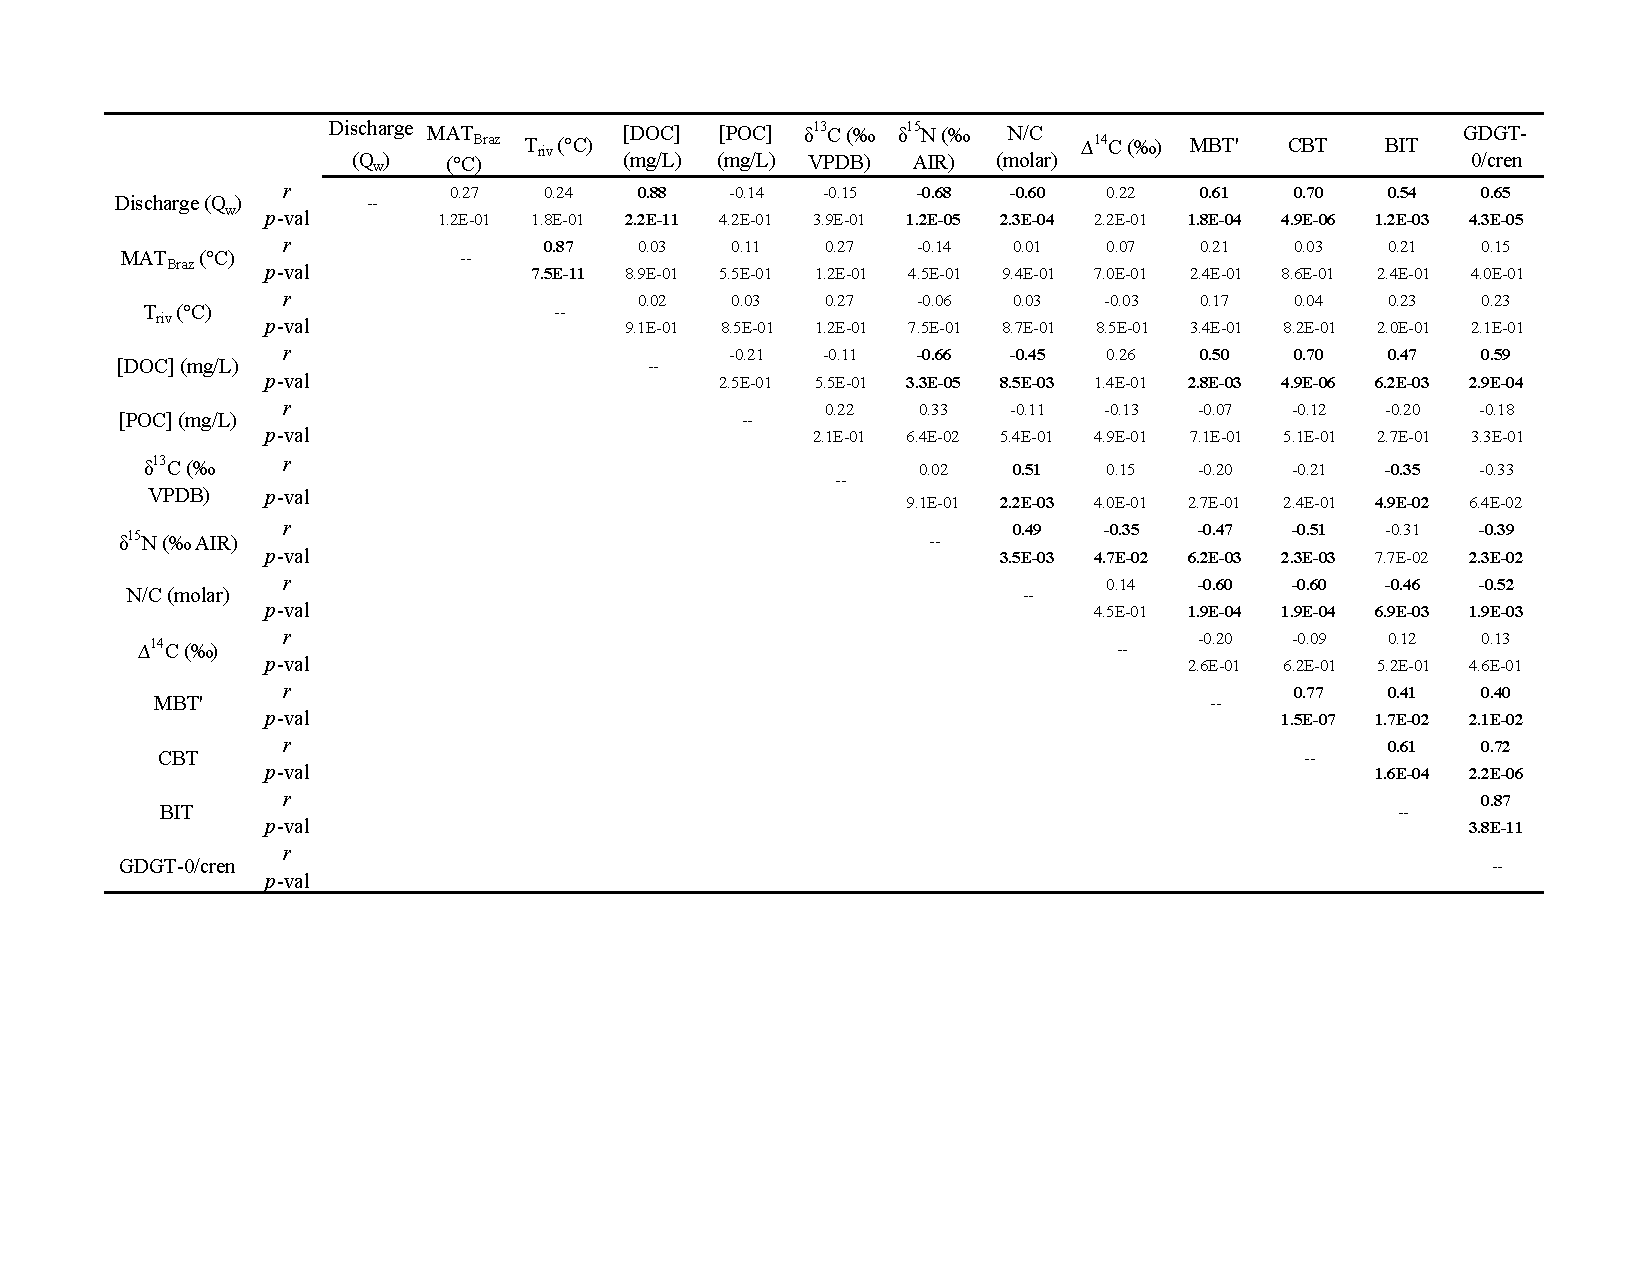
\includegraphics{Thesis_Tables/Ch5Tab2}
	\label{Ch5Tab:2} 
\end{sidewaystable}

\subsection{Bulk measurements}

\subsubsection{DOC and POC concentrations}

Congo River [DOC] ranges from $5.1$ mg L\textsuperscript{-1} in June 2011 to $14.2$ mg L\textsuperscript{-1} in October 2012 (mean = $9.0 \pm 2.5$ mg L\textsuperscript{-1}; Figure \ref{Ch5Fig:2}E) and exhibits significant correlations with Q\textsubscript{w} (positive), \ce{\delta^{15}N} (negative), N/C (negative), and all GDGT metrics (all positive; Table \ref{Ch5Tab:2}). POC concentration ([POC]) ranges from a minimum of $0.6$ mg L\textsuperscript{-1} in August 2013 to a maximum of $2.6$ mg L\textsuperscript{-1} in February 2011 \citep[mean = $1.3 \pm 0.4$ mg L\textsuperscript{-1}; Figure \ref{Ch5Fig:2}F;][]{Hemingway:2016bq} and is uncorrelated with all environmental parameters, bulk measurements, and GDGT metrics (Table \ref{Ch5Tab:2}). For the Djoue River time-series, [POC] ranges from $0.6$ mg L\textsuperscript{-1} in August 2011 to $1.1$ mg L\textsuperscript{-1} in April, June, and November 2011 (mean = $0.9 \pm 0.2$ mg L\textsuperscript{-1}). Unlike the Congo River, Djoue [POC] exhibits a statistically significant positive correlation with bulk \ce{\delta^{13}C} ($r = 0.60$, $p$-value = $3.05 \times 10^{-2}$, $n = 13$; not shown).

\subsubsection{Stable isotope (\ce{^{13}C}, \ce{^{15}N}) and N/C composition}

\ce{\delta^{13}C} values of Congo River POC across the time-series range from $-27.6$\textperthousand\ (November--December 2010) to $-24.6$\textperthousand\ (February 2013), averaging $-26.4 \pm 0.7$\textperthousand\ (Figure \ref{Ch5Fig:3}A). Additionally, \ce{\delta^{13}C} values exhibit a statistically significant positive relationship with N/C and a negative relationship with BIT (Table \ref{Ch5Tab:2}). Djoue River POC \ce{\delta^{13}C} values are statistically identical to those of the Congo River, with a range of $-28.1$\textperthousand\ (August 2011) to $-26.5$\textperthousand\ (April 2011) and a mean of $-27.5 \pm 0.5$\textperthousand.

The nitrogen stable isotope composition of Congo River POM is slightly more variable than that of carbon, with \ce{\delta^{15}N} values ranging from $3.9$\textperthousand\ (December 2012--January 2013) to $8.5$\textperthousand\ (August 2011; mean = $6.1 \pm 1.1$\textperthousand; Figure \ref{Ch5Fig:3}B). \ce{\delta^{15}N} values display a strong negative correlation with both Q\textsubscript{w} and [DOC], as well as weaker correlations with N/C (positive), \ce{\Delta^{14}C} (negative), MBT', CBT, and GDGT-0/cren (all negative; Table \ref{Ch5Tab:2}). As with \ce{\delta^{13}C}, Djoue River \ce{\delta^{15}N} values span a similar range as those of the Congo River ($3.8$\textperthousand\ in December 2010 to $6.4$\textperthousand\ in August 2011), with a mean value of $5.0 \pm 0.7$\textperthousand.

Congo River N/C ranges from $0.076$ (December 2010) to $0.118$ (August 2012) with an average of $0.096 \pm 0.010$ (Figure \ref{Ch5Fig:3}C). Like \ce{\delta^{15}N} values, N/C displays a negative correlation with Q\textsubscript{w} and [DOC], and is additionally negatively correlated with all GDGT metrics and positively correlated with \ce{\delta^{13}C} and \ce{\delta^{15}N} (Table \ref{Ch5Tab:2}). Unlike stable isotopes, the Djoue River time-series average N/C value is statistically lower than that of the Congo River ($p$-value = $1.10 \times 10^{-2}$), with individual samples ranging from a minimum of $0.050$ (January, May 2011) to a maximum of $0.080$ (April 2011; mean = $0.065 \pm 0.010$).

% Figure 3
\begin{figure}[ht]
	\makebox[\textwidth][c]{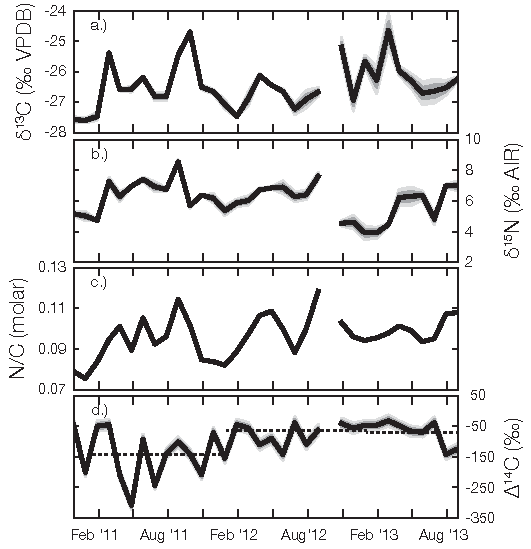
\includegraphics[]{Thesis_Figures/Ch5Fig3}}
	\caption[Bulk parameter time-series plots]{Time-series plots of Congo River bulk POM molecular and isotopic composition: $(A)$ \ce{\delta^{13}C}, $(B)$ \ce{\delta^{15}N}, $(C)$ N/C, and $(D)$ \ce{\Delta^{14}C}. Where visible, dark gray envelope is $\pm 1 \sigma$ uncertainty and light gray envelope is 95\% confidence interval. Dotted lines in panel $(D)$ are the flux-weighted-average values for each calendar year (January--August only for 2013).}
	\label{Ch5Fig:3} 
\end{figure}

\subsubsection{\ce{^{14}C} composition}

Radiocarbon composition of exported Congo River POC is highly variable, with \ce{\Delta^{14}C} ranging from $-309$\textperthousand\ in April 2011 to $-33$\textperthousand\ in February 2013 (mean = $-105 \pm 69$\textperthousand; Figure \ref{Ch5Fig:3}D). Because \ce{\Delta^{14}C} is more depleted and variable during 2011 as opposed to 2012 and 2013, there exists a statistically significant positive temporal trend throughout the time-series, with an increase of $32.5$\textperthousand/year ($r = 0.39$, $p$-value = $2.80 \times 10^{-2}$). Additionally, \ce{\Delta^{14}C} displays a slight negative correlation with \ce{\delta^{15}N} as described above, but is uncorrelated with all other environmental variables, bulk measurements, and GDGT metrics (Table \ref{Ch5Tab:2}).

\subsection{GDGT distributions}

Homologue brIa is the most abundant brGDGT throughout the time-series, contributing between $73$ and $82$\% of total brGDGTs (mean = $77 \pm 2$\%; Table \ref{Ch5Tab:S2}). Homologues brIIa (mean = $14 \pm 1$\%) and brIb (mean = $5 \pm 1$\%) are consistently the second- and third-most abundant branched homologues, respectively. All remaining branched homologues contribute $1-2$\% of the brGDGT total, with the exception of brIIIc which was not detected in any sample. This leads to an MBT' range of $0.80 - 0.86$ (mean = $0.84 \pm 0.01$) and a CBT range of $1.00 - 1.32$ (mean = $1.15 \pm 0.08$; Figure \ref{Ch5Fig:4}A, Figure \ref{Ch5Fig:4}B). IsoGDGTs are significantly less abundant than branched compounds, with total isoGDGTs (crenarchaeol and GDGT-0 only) comprising between $5$ and $10$\% of the brGDGT total (mean = $6 \pm 1$\%). Resulting in BIT values are consistently $\geq 0.96$ (Figure \ref{Ch5Fig:4}C). With the exception of July and August 2013, GDGT-0 is more abundant than crenarchaeol, comprising $60 \pm 6$\% of isoGDGTs, and resulting in a GDGT-0/cren ratio ranging from $0.7$ to $2.4$ (mean = $1.6 \pm 0.4$; Figure \ref{Ch5Fig:4}D). All GDGT metrics are positively correlated with each other and exhibit strong positive correlations with Q\textsubscript{w} and [DOC], as well as negative correlations with \ce{\delta^{15}N} (excluding BIT) and N/C (Table \ref{Ch5Tab:2}).

% Figure 4
\begin{figure}[ht]
	\makebox[\textwidth][c]{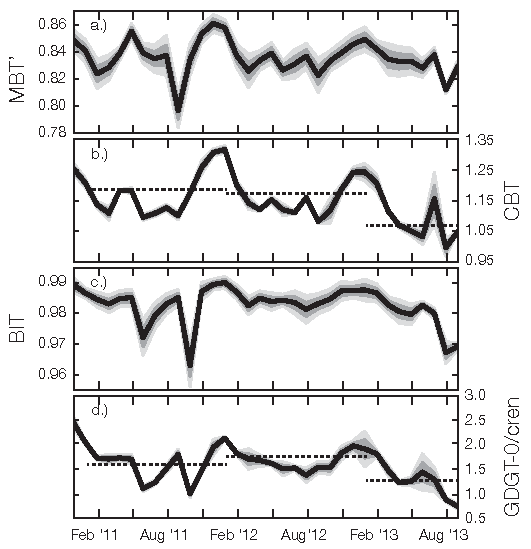
\includegraphics[]{Thesis_Figures/Ch5Fig4}}
	\caption[GDGT metric time-series plots]{Time-series plots of Congo River GDGT distribution metrics: $(A)$ MBT', $(B)$ CBT, $(C)$ BIT, and $(D)$ GDGT-0/cren. Where visible, dark gray envelope is $\pm 1 \sigma$ uncertainty and light gray envelope is 95\% confidence interval. Dotted lines in panels $(B)$ and $(D)$ are the flux-weighted-average values for each calendar year (January--August only for 2013).}
	\label{Ch5Fig:4} 
\end{figure}

\section{Discussion}

\subsection{OC fluxes, yield, and the importance of the \textit{Cuvette Congolaise}}

Congo River [POC] in our dataset is in good agreement with previously published values from nearby sampling sites \citep{Mariotti:1991vx,Coynel:2005cn,Spencer:2012en,Spencer:2016ho}. The time-series average reported here (mean = $1.3 \pm 0.4$ mg L\textsuperscript{-1}) is slightly lower than that of \citet{Mariotti:1991vx} from the years 1976 and 1983 (mean = $2.0 \pm 0.2$ mg L\textsuperscript{-1}, $n = 10$) and of \citet{Coynel:2005cn} from the years 1990--1993 (mean = $1.74$ mg L\textsuperscript{-1}, $n = 23$), but is similar to the recent measurements of \citet{Spencer:2012en,Spencer:2016ho} (mean = $1.5 \pm 0.3$ mg L\textsuperscript{-1}, $n = 19$). While less data exist for the Djoue River, [POC] from our time-series is nearly identical to that of \citet{Mariotti:1991vx} (mean = $0.7 \pm 0.1$ mg L\textsuperscript{-1}, $n = 3$).

Suspended sediment export from the Congo River, both in terms of TSS concentration and yield, is significantly lower than for other large temperate and tropical rivers across the globe \citep{Ludwig:1998ud,Milliman:2011ug,Galy:2015fx}. However, TSS exhibit high \%OC values leading to [POC] near that of other tropical rivers such as the Amazon \citep{Richey:1990wl}. Calculated POC yield using our time-series is $0.42 \pm 0.004$ tC km\textsuperscript{-2} yr\textsuperscript{-1} between November 2010 and August 2013, slightly lower than previously published values of $0.68$ tC km\textsuperscript{-2} yr\textsuperscript{-1} \citep{Ludwig:1996ul} and $0.55$ tC km\textsuperscript{-2} yr\textsuperscript{-1} \citep{Coynel:2005cn,Spencer:2016ho}. Annual POC yield for the entire Congo basin is greater than that of the Oubangui sub-basin ($0.26$ tC km\textsuperscript{-2} yr\textsuperscript{-1}) due to the fact that northern-hemisphere summer base-flow conditions lead to reduced Oubangui River POC fluxes \citep{Bouillon:2012cw}.

While most rivers display clear positive, nonlinear relationships between discharge, TSS yield, and POC yield (\textit{i.e.} rating curves), such trends are significantly weaker in the Congo River due to a lack of correlation between Q\textsubscript{w} and [POC] (Table \ref{Ch5Tab:2}). This result is at least partially due to hysteresis effects. Highest [POC] is generally observed during the rising limb of the hydrograph (Sep-Oct-Nov) due to the flushing of sediments previously entrained in the \textit{Cuvette Congolaise}, while the falling limb (Dec-Jan-Feb) exhibits lower [POC] for similar discharge values \citep{Spencer:2016ho}. Furthermore, during boreal spring and summer when water flux through this region is low and non-erosive \citep{Bricquet:1993ve,Henchiri:2016jh}, the \textit{Cuvette Congolaise} acts as sediment trap, removing POM derived from right-bank and main-stem headwaters \citep{Laraque:2009fz}.

In contrast to POC, Congo River DOC follows typical rating curve behavior due to the strong positive correlation between Q\textsubscript{w} and [DOC] (Table \ref{Ch5Tab:2}), as has been reported previously \citep{Coynel:2005cn,Wang:2013js,Spencer:2016ho}. Still, [DOC] does display a slight hysteresis effect, with highest concentrations observed during the rising limb of the hydrograph (Sep-Oct-Nov). This result is again due to flushing of \textit{Cuvette}-derived DOC at this time, as swamp-forest tributaries within the Congo basin have been shown to reach [DOC] values as high as $\approx 80$ mg L\textsuperscript{-1} \citep{Mann:2014jx}. Resulting DOC yield over the course of our time-series is $3.11 \pm 0.03$ tC km\textsuperscript{-2} yr\textsuperscript{-1}, leading to a dissolved-phase contribution to total exported OC of $87 \pm 5$\%. Annual yield calculated here is within the range of previously reported estimates [$2.47$ tC km\textsuperscript{-2} yr\textsuperscript{-1} \citep{Ludwig:1996ul}, $3.44$ tC km\textsuperscript{-2} yr\textsuperscript{-1} \citep{Coynel:2005cn}, $3.48$ tC km\textsuperscript{-2} yr\textsuperscript{-1} \citep{Spencer:2016ho}], and is roughly double that of the Oubangui sub-basin [$1.43$ tC km\textsuperscript{-2} yr\textsuperscript{-1} \citep{Bouillon:2012cw}].

\subsection{Congo River POM sources: Insight from bulk measurements}

Like concentration and flux results, Congo River POM isotope and N/C composition presented here agrees with previously published values from nearby sampling sites \citep{Mariotti:1991vx,Spencer:2012en,Spencer:2016ho}. While our results represent OM contained in bulk TSS, they are nearly identical to published results from the fine fraction only ($<63 \mu$m), as this contains $>80$\% of total POM \citep{Spencer:2012en}. In contrast, coarse material ($\geq63 \mu$m) has been shown to display significantly lower N/C ratios (Figure \ref{Ch5Fig:5}A) as well as \ce{\Delta^{14}C} values $>0$\textperthousand\ due to incorporation of bomb-derived \ce{^{14}C} (Figure \ref{Ch5Fig:5}B), and has been interpreted as representing recently fixed rainforest vegetation and plant debris \citep{Spencer:2012en}. 

% Figure 5
\begin{figure}[p]
	\makebox[\textwidth][c]{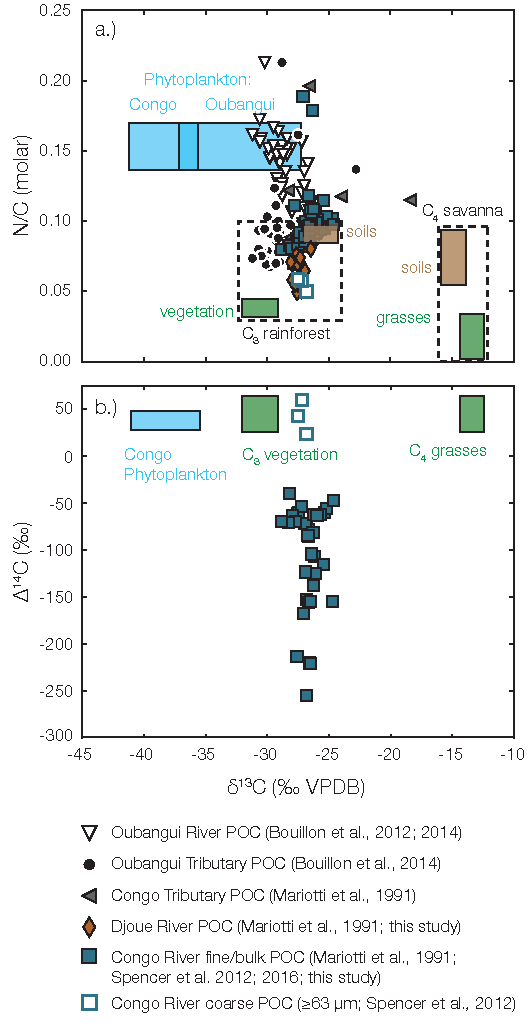
\includegraphics[]{Thesis_Figures/Ch5Fig5}}
	\caption[Conservative tracer mixing model]{Conservative tracer mixing model plots showing all published POM data from within the Congo basin: $(A)$ \ce{\delta^{13}C} vs. N/C and $(B)$ \ce{\delta^{13}C} vs. \ce{\Delta^{14}C}. End-member compositions are listed in Table \ref{Ch5Tab:3} and described in section \ref{Ch5SD2}.}
	\label{Ch5Fig:5} 
\end{figure}

Generally, Congo River main-stem POM is more enriched in \ce{^{13}C} and depleted in N/C relative to the Oubangui River during similar discharge regimes \citep[Figure \ref{Ch5Fig:6}A--B;][]{Bouillon:2012cw,Bouillon:2014ko} and plots within the C\textsubscript{3} rainforest end-member range (Table \ref{Ch5Tab:3}; Figure \ref{Ch5Fig:5}A; see Supplemental Discussion \ref{Ch5SD2} on end-member compositions), indicating that headwater material is diluted and/or replaced during transit through the \textit{Cuvette Congolaise}. Furthermore, predominantly C\textsubscript{4}-savanna-derived POM is never observed (Figure \ref{Ch5Fig:5}A) despite large regions of C\textsubscript{4} landcover, especially in southern-hemisphere tributary and Djoue River catchments (Table \ref{Ch5Tab:1}; Figure \ref{Ch5Fig:1}B). This agrees with the \ce{^{13}C} composition of plant-wax \textit{n}-alcohols and \textit{n}-alkanoic acids \citep{Hemingway:2016bq} and the molecular composition of lignin phenols \citep{Spencer:2016ho} extracted from Congo River TSS, which preclude large C\textsubscript{4}-grass inputs to these biomarker classes. However, left-bank tributaries such as the Kasai River exhibit the highest TSS yield within the Congo basin \citep{Laraque:2009fz}, suggesting that a non-negligible fraction of exported POM is derived from this region, except during 2011 when southern-hemisphere discharge was anomalously low (Figure \ref{Ch5Fig:2}A). The lack of significant C\textsubscript{4} contribution observed throughout our Congo River and Djoue River time-series likely supports the idea that exported bulk POM signals bias toward riparian zones \citep{Bouillon:2012cw}, as these regions are dominated by C\textsubscript{3} landcover throughout the basin (Figure \ref{Ch5Fig:1}). However, we note that, in contrast to all other signals, \ce{^{13}C}-enriched C\textsubscript{33} and C\textsubscript{35} \textit{n}-alkanes have been observed in the Congo River, indicating the persistence of distal C\textsubscript{4} inputs to these low concentration, recalcitrant biomarkers \citep{Hemingway:2016bq}.

% Table 3
\begin{sidewaystable}[p]
	\caption[Mixing model end-member compositions]{Mixing model end-member compositions. See section \ref{Ch5SD2} for further discussion.}
	\centering
		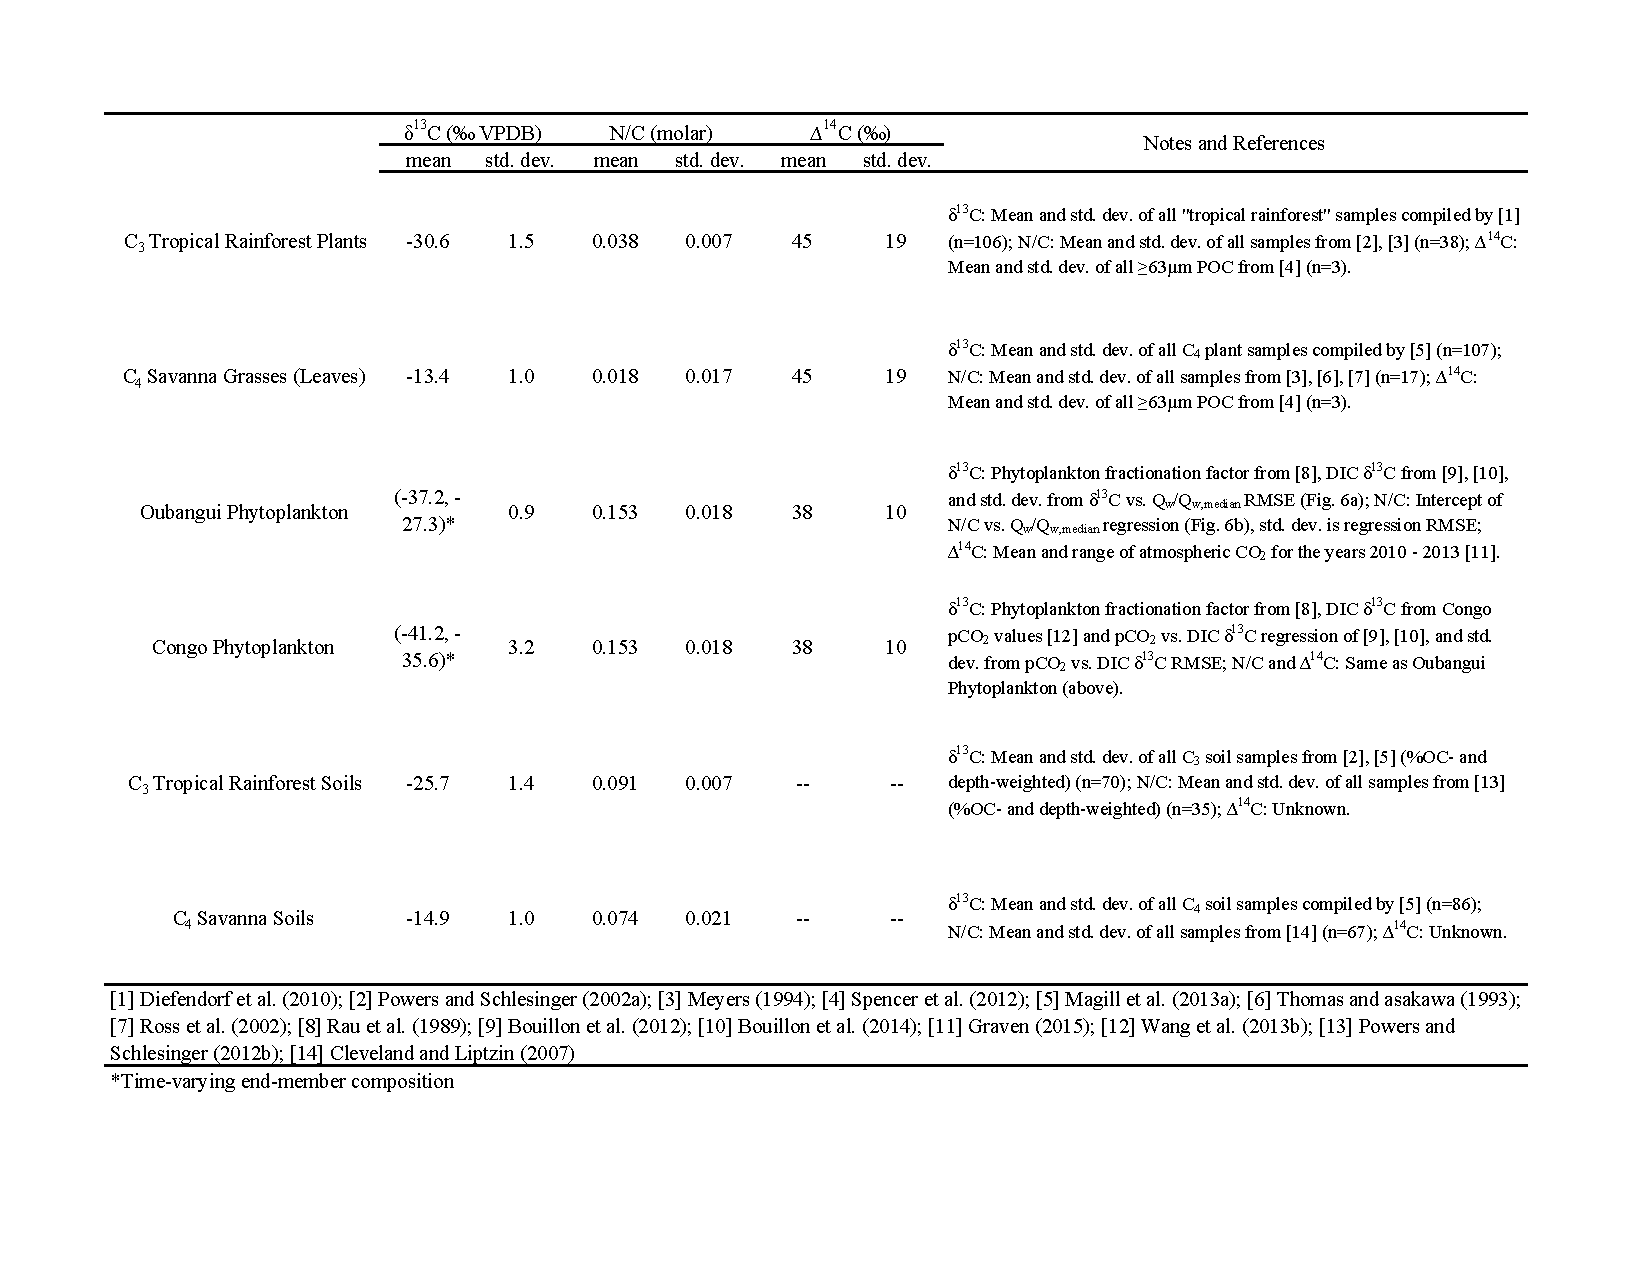
\includegraphics{Thesis_Tables/Ch5Tab3}
	\label{Ch5Tab:3} 
\end{sidewaystable}

Additionally, significant OC\textsubscript{petro} erosion in the Congo basin is unlikely due to the low catchment relief and lack of OC-rich bedrock lithology \citep{Copard:2007bf,Milliman:2011ug}. We therefore omit C\textsubscript{4}-savanna and OC\textsubscript{petro} sources form our mixing model and quantitatively calculate the contributions of C\textsubscript{3} tropical rainforest vegetation, C\textsubscript{3} tropical rainforest soils, and autochthonous phytoplankton to Congo River \citep[][this study]{Spencer:2016ho} and Oubangui River POM \citep{Bouillon:2012cw,Bouillon:2014ko}. We retain \ce{\delta^{13}C} and N/C as conservative tracers, as \ce{\Delta^{14}C} of eroded soils is highly variable and difficult to constrain \textit{a priori}, while absolute \ce{\delta^{15}N} values of vegetation, soils, and phytoplankton are influenced by unknown nitrogen sources, fixation pathways, and (re)cycling \citep{Martinelli:1999ta,Kendall:2001bs}. Resulting end-member contributions are reported in Table \ref{Ch5Tab:S3}. 

% Figure 6
\begin{figure}[p]
	\makebox[\textwidth][c]{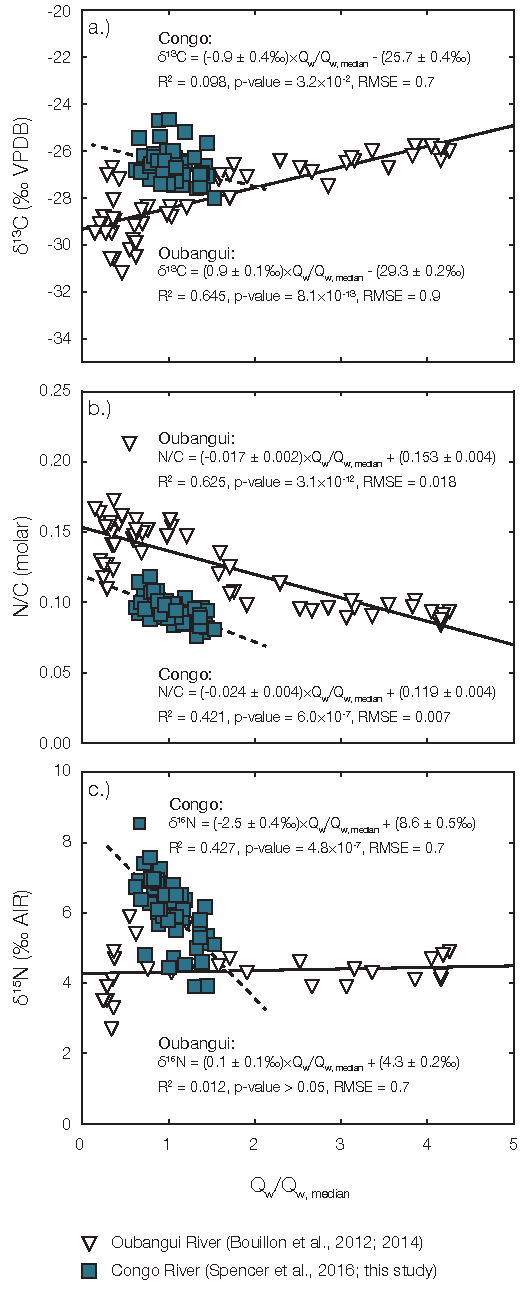
\includegraphics[scale=0.9]{Thesis_Figures/Ch5Fig6}}
	\caption[Discharge vs. \ce{\delta^{13}C}, N/C, and \ce{\delta^{15}N}]{Correlations between Congo River and Oubangui River discharge vs. $(A)$ \ce{\delta^{13}C}, $(B)$ N/C, and $(C)$ \ce{\delta^{15}N}. To present both records on the same scale, discharge has been normalized by the median discharge value for each time-series (Q\textsubscript{w}/Q\textsubscript{w, median}).}
	\label{Ch5Fig:6} 
\end{figure}

\subsubsection{Seasonal source variability}

Congo River POM at Brazzaville/Kinshasa is consistently dominated by C\textsubscript{3} soil material (median = $87$\%, inter-quartile range = $80 - 91$\%; Figure \ref{Ch5Fig:7}A), with low contribution by C\textsubscript{3} tree litter (median = $1$\%, inter-quartile range = $0 - 13$\%; Figure \ref{Ch5Fig:7}B) and autochthonous phytoplankton production (median = $8$\%, inter-quartile range = $6 - 11$\%; Figure \ref{Ch5Fig:7}C). In contrast, Oubangui River POM is composed almost entirely of C\textsubscript{3} rainforest soils when discharge is high (median = $33$\%, inter-quartile range = $8 - 86$\%; Figure \ref{Ch5Fig:7}A) and phytoplankton sources during base-flow conditions (median = $62$\%, inter-quartile range = $11 - 92$\%; Figure \ref{Ch5Fig:7}C), with minimal contribution by C\textsubscript{3} rainforest vegetation throughout the hydrograph (median = $0$\%, inter-quartile range = $0 - 2$\%; Figure \ref{Ch5Fig:7}B). 

Seasonal importance of phytoplankton-derived POM in the Oubangui River therefore does not propagate to the main-stem Congo River at Brazzaville/Kinshasa (Figure \ref{Ch5Fig:7}C) due to a combination of: $(i)$ dilution by downstream inputs, $(ii)$ remineralization during transit, and/or $(iii)$ loss due to particle settling/trapping within the \textit{Cuvette Congolaise} when water flux through this region is low \citep{Laraque:2009fz}. However, while low throughout the time-series, phytoplankton contribution to Congo River POM does display a statistically significant decrease with increasing discharge ($r = -0.60$, $p$-value = $6.10 \times 10^{-6}$, $n = 48$; Figure \ref{Ch5Fig:7}C). This result agrees with observed seasonal trends in C\textsubscript{24} \textit{n}-alcohol \ce{^{13}C} composition, as this compound has been shown to be influenced by autochthonous production \citep{Hemingway:2016bq}.

Unlike phytoplankton, C\textsubscript{3} vegetation contribution to POC is typically higher in the Congo River main-stem than in the Oubangui River and is positively correlated with discharge ($r = 0.57$, $p$-value = $1.98 \times 10^{-5}$, $n = 48$; Figure \ref{Ch5Fig:7}B), reflecting increasing admixture of less degraded vascular plant material when water flux through the \textit{Cuvette Congolaise} is high. While absolute end-member \ce{\delta^{15}N} values are difficult to constrain \textit{a priori}, a compilation of tropical rainforest samples indicates that fresh vegetation is depleted in \ce{^{15}N} by $6.9 \pm 4.5$\textperthousand\ relative to soils \citep{Martinelli:1999ta}. In contrast, \ce{\delta^{15}N} of Oubangui River POM is constant across the hydrograph (Figure \ref{Ch5Fig:6}C) and suggests that this tracer is insensitive to phytoplankton vs. C\textsubscript{3}-soil inputs in this system, although we note that Congo River POM end-member compositions are likely not identical to those in the Oubangui. Still, the strong negative correlation between Congo River POM \ce{\delta^{15}N} and discharge observed here (Figure \ref{Ch5Fig:6}C) is further evidence for an increase in fresh vascular plant material with increasing discharge. This result is additionally supported by observed seasonal variability in the chemical composition and carbon-normalized yield of particulate lignin phenols, which shift toward higher yield and less degraded signatures when discharge is high \citep{Spencer:2016ho}.

% Figure 7
\begin{figure}[p]
	\makebox[\textwidth][c]{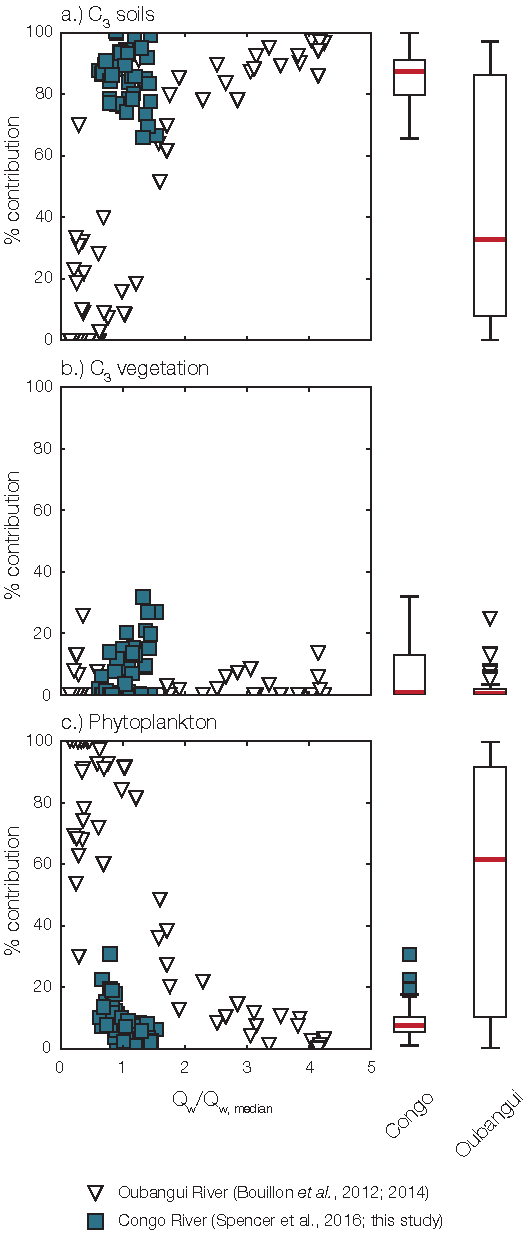
\includegraphics[scale=0.9]{Thesis_Figures/Ch5Fig7}}
	\caption[Discharge vs. end-member fractional contribution]{Fractional contribution box plots and correlations with discharge for: $(A)$ C\textsubscript{3} soils, $(B)$ C\textsubscript{3} vegetation, and $(C)$ phytoplankton. To present both records on the same scale, discharge has been normalized by the median discharge value for each time-series (Q\textsubscript{w}/Q\textsubscript{w, median}). For box plots, red lines are median values, boxes contain the inter-quartile range, and whiskers contain the 95\% confidence interval. Individual outliers are plotted as blue squares (Congo) and white triangles (Oubangui).}
	\label{Ch5Fig:7} 
\end{figure}

\subsubsection{Controls on soil \ce{\Delta^{14}C}}

While consistently dominated by C\textsubscript{3}-soil material, the \ce{^{14}C} composition of exported Congo River POC is highly variable, especially in 2011 when southern-hemisphere discharge was lowest (Figure \ref{Ch5Fig:3}D). Observed \ce{\Delta^{14}C} values cannot be explained by OC\textsubscript{petro} inputs due to low erosion rates and a lack of OC-rich bedrock in the Congo basin \citep{Copard:2007bf}, and are therefore interpreted to reflect variable ages of eroded soils. We calculate the \ce{^{14}C} composition of exported soil-derived POC using the equation:

% Equation 4
\begin{equation}\label{Ch5Eq:4}
	\ce{\Delta^{14}C}_{\text{soil}} = \frac{1}{f_{\text{soil}}} \left(\ce{\Delta^{14}C}_{\text{POC}} - f_{\text{phyto}}\ce{\Delta^{14}C}_{\text{phyto}} - f_{\text{plants}}\ce{\Delta^{14}C}_{\text{plants}} \right)
\end{equation}

where $f_i$ is the calculated fractional contribution of end member $i$ (Table \ref{Ch5Tab:S3}), \ce{\Delta^{14}C}\textsubscript{POC} is the measured POC \ce{\Delta^{14}C} value (Table \ref{Ch5Tab:S1}), and \ce{\Delta^{14}C}\textsubscript{phyto} and \ce{\Delta^{14}C}\textsubscript{plants} are phytoplankton and C\textsubscript{3} tropical rainforest vegetation end-member values (Table \ref{Ch5Tab:3}; Figure \ref{Ch5Fig:5}B). 

Eroded soil-derived POC exhibits low and variable \ce{\Delta^{14}C} values during 2011 (annual mean = $-176 \pm 93$\textperthousand) as compared to 2012 (annual mean = $-90 \pm 39$\textperthousand) and 2013 (Jan--Aug mean = $-85 \pm 53$\textperthousand), suggesting that anomalously low southern-hemisphere discharge in 2011 resulted in a bias toward export of pre-aged, \textit{Cuvette}-derived soils at this time. In contrast, \ce{\Delta^{14}C} values of soil-derived POC were near $-50$\textperthousand\ from January to June 2013, when left-bank tributary discharge peaked above the 1977--2006 average for these months (Figure \ref{Ch5Fig:2}A). Ecosystems drained by left-bank tributaries in the Congo basin (grassland, woodland/shrubland, Figure \ref{Ch5Fig:1}A) are highly productive with most biomass being produced as leaves and foliage \citep{Bloom:2016gm}, resulting in a large carbon input flux to soils and thus short soil residence times \citep{Carvalhais:2014dc}. Combined with relatively high TSS yields in these tributaries \citep{Laraque:2009fz}, this supports our interpretation that increased precipitation and discharge in the southern half of the basin leads to higher \ce{^{14}C} content of exported soil-derived POC.

Furthermore, increased terrestrial reservoir ages (\textit{i.e.} lower \ce{^{14}C} composition relative to the atmosphere at the time of deposition) since the Early- to Mid-Holocene have been observed in plant-wax lipids, wood pieces, and OC extracted from Congo Fan sediments, concomitant with decreasing precipitation intensity at this time \citep{Schefuss:2005jo}, and have been interpreted as reflecting erosion of pre-aged, previously inundated \textit{Cuvette Congolaise} swamp deposits \citep{Schefuss:2016cp}. These results indicate that \textit{Cuvette}-derived POM contains eroded soils with lower \ce{^{14}C} content than those sourced from other ecosystems within the basin, likely due to efficient OC preservation under permanently inundated, anoxic conditions. The time-series \ce{\Delta^{14}C} results presented here further support this idea, and show that relative changes in \textit{Cuvette Congolaise} inputs leads to variability in exported POC ages on inter-annual timescales in addition to the millennial-timescale variability described in \citet{Schefuss:2016cp}. Thus, if the observed decreases in Apr-May-Jun precipitation in the Congo basin over the past decade continue \citep{Zhou:2014gl}, our data suggest that exported soil-derived POM will further bias toward protracted \textit{Cuvette Congolaise} sources under future discharge regimes. Because OM stored under anoxic conditions has been shown to be highly susceptible to degradation upon exposure to O2 \citep{Hoefs:2002wu}, increasing relative contribution by this end-member to exported POM could additionally result in increased remineralization during fluvial transit.

\subsection{Congo River POM sources: Insight from GDGT metrics}

Congo River GDGTs can provide further information regarding POM provenance, especially since variability in material sourced from the highly acidic, anoxic \textit{Cuvette Congolaise} \citep{Mann:2014jx} should be reflected in CBT and GDGT-0/cren metrics \citep{Blaga:2009ge,Peterse:2012bs}. Indeed, these indices display large variability throughout the time-series (Figure \ref{Ch5Fig:4}B, D), indicating significant seasonal changes in GDGT source. Although GDGT distributions for each end member could not be measured directly, redundancy analysis \citep[RDA;][]{Legendre:1998tt} indicates that a majority of variance in GDGT metrics can be described by a canonical axis that is strongly correlated with hydrology (Table \ref{Ch5Tab:S4}; Figure \ref{Ch5Fig:8}). Analagous to bulk POM results, this suggests a hydrologic control on GDGT sources and molecular distributions in Congo River TSS. 

It is possible that seasonal variability is due to \textit{in situ} brGDGT production within the river when discharge is low, as this would lead to the observed decreases in MBT' and CBT at this time \citep{Peterse:2009hl,Tierney:2010br} and has previously been invoked to explain brGDGT distributions in other river systems \citep{DeJonge:2014fs,Zell:2014gt}. However, significant \textit{in situ} brGDGT production within the water column on seasonal timescales is unlikely, as these compounds have been shown to exhibit much longer growth times. For example, \citet{Peterse:2015ef} observed no \textit{in situ} production of intact polar brGDGTs in 160-day incubations of TSS from New Zealand rivers. While the incubation conditions of \citet{Peterse:2015ef} are not identical to those within the Congo River, significant autochthonous production would additionally lead to bulk N/C enrichment and \ce{^{13}C} depletion during low discharge, which is clearly not observed (Figure \ref{Ch5Fig:3}A, \ref{Ch5Fig:3}C).

% Figure 8
\begin{figure}[ht ]
	\makebox[\textwidth][c]{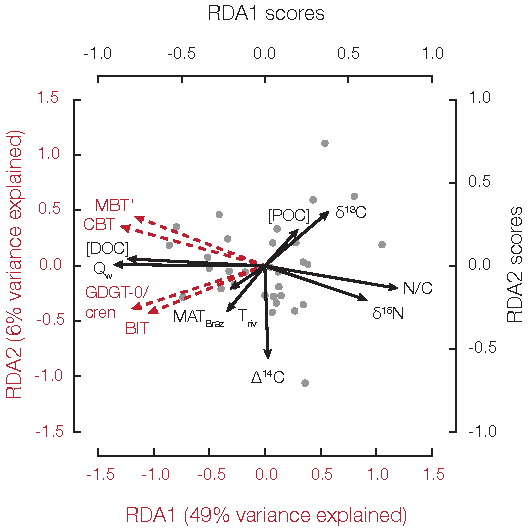
\includegraphics[]{Thesis_Figures/Ch5Fig8}}
	\caption[Environmental parameter, bulk metrics, and GDGT distribution RDA analysis]{Congo River time-series RDA triplot ("Type III" scaling) showing the first (RDA1) and second (RDA2) canonical axes. Environmental variable scores are plotted as black arrows, response variable ("species") scores are plotted as red dashed arrows, and individual sample ("site") scores are plotted as gray circles. Red axes labels correspond to response variable scores while black axes labels correspond to environmental variable scores.}
	\label{Ch5Fig:8} 
\end{figure}

Rather, variability is likely due to incorporation of GDGTs produced in permanently inundated, anoxic \textit{Cuvette Congolaise} soils when discharge through this region is high. This is supported by the observation that water-logged, acidic soils in western Uganda exhibit significantly higher CBT values than well-drained, aerobic soils from the same transect \citep{Loomis:2011dr}. Similarly, water-saturated and oxygen-depleted peat bogs have been shown to display higher CBT values than nearby aerobic sites \citep{Huguet:2010di}, as dissolved oxygen content has been shown to exert a strong control on bacterial community composition \citep{Hansel:2008hp} and likely brGDGT distributions. In our time-series, flux-weighted-average CBT during 2013 is significantly lower than in 2011 and 2012 (Figure \ref{Ch5Fig:4}B), consistent with elevated southern-hemisphere discharge and increased contribution by left-bank POM in 2013.

Additionally, GDGT-0/cren ratios $>2$ are generally thought to represent substantial contribution by anaerobic methanogenic archaea \citep{Blaga:2009ge}. Significant methanogenesis in \textit{Cuvette Congolaise} soils is indirectly supported by the high concentrations and \ce{^{13}C} composition of amino-bacteriohopanepolyls in this region \citep{Talbot:2014jd,SpencerJones:2015bn}. Therefore, in addition to higher CBT values, increased incorporation of GDGTs from swamp-forest soils during high discharge should lead to elevated GDGT-0/cren ratios, as is observed (Figure \ref{Ch5Fig:4}D). Similar to CBT, flux-weighted-average GDGT-0/cren is lowest in 2013 as compared to 2011 and 2012, further supporting the idea that increased left-bank contribution is the source of exported POM with higher \ce{^{14}C} content and less acidic/methanogenic GDGT sources at this time. In contrast, low southern-hemisphere discharge in 2011, and to a lesser degree in 2012 (Figure \ref{Ch5Fig:2}A), leads to exported POM that is biased toward pre-aged \textit{Cuvette Congolaise} soils. Thus, GDGT metrics agree with bulk end-member mixing-model and \ce{\Delta^{14}C} results in highlighting the importance of the \textit{Cuvette Congolaise} in determining exported POM signals from the Congo River.

\section{Conclusion}

We present a 34-month record of Congo River DOC concentrations, POM composition (\ce{\delta^{13}C}, \ce{\delta^{15}N}, \ce{\Delta^{14}C}, N/C), and GDGT distributions to constrain seasonal and inter-annual variability in the source of exported OM. Our results indicate that all Congo River POM samples are consistently dominated by C\textsubscript{3} soil inputs throughout the time-series, with decreasing contribution by phytoplankton and increasing contribution by fresh C\textsubscript{3} vegetation during high discharge. In contrast, large inputs by C\textsubscript{4} grasses are never observed.

Exported soil-derived POC displays low and variable \ce{^{14}C} content, especially during 2011 when southern-hemisphere discharge was anomalously low. Combined with higher CBT and GDGT-0/cren values in 2011, this suggests that acidic, anoxic \textit{Cuvette Congolaise} soils are an important source of pre-aged OM to the Congo River. Furthermore, high southern-hemisphere discharge in spring 2013 coincides with stable, high \ce{^{14}C} content and suggests that left-bank tributaries are a source of young soil-derived POM, consistent with lower CBT and GDGT-0/cren at this time.

This study demonstrates that POM exported from tropical, wet river catchments can contain significantly pre-aged biospheric material due to protracted storage in anoxic soils. We emphasize that permanently inundated areas such as those present in the \textit{Cuvette Congolaise} are an important OM reservoir despite their relatively small landcover extent and could be more significant in determining the role of tropical rivers in the global carbon cycle than previously thought, especially if future hydrologic regimes favor export and remineralization of this material.

%\section*{Acknowledgements}
%We thank Carl Johnson (WHOI), Ekaterina Bulygina (Woods Hole Research Center), Sarah Rosengard (WHOI), Helena Pryer (WHOI), Negar Haghipour (ETH), and Lukas Wacker (ETH) for laboratory assistance. V.V.G. was partly supported by the US National Science Foundation, grants OCE-0851015 and OCE-0928582; J.D.H. was supported by the NSF Graduate Research Fellowship Program under grant number 2012126152; T.I.E. was partly supported by the Swiss National Science Foundation (SNF Grant No. 200021 140850); E.S. was supported by the DFG Research Center/Cluster of Excellence "The Ocean in the Earth System" at MARUM--Center for Environmental Sciences; R.G.M.S. was partly supported by the US National Science Foundation, grants ETBC-0851101, OCE-1333157, and OCE-1464396.

\clearpage

\section{Supplementary Material}

\subsection{Discussion}

\subsubsection{Effect of 6-methyl brGDGTs}\label{Ch5SD1}

Updated chromatographic methods not employed here now allow for the separation of previously co-eluting 5-methyl and 6-methyl brGDGTs and have led to improved metrics for tracking environmental parameters when calibrated using a global soil dataset \citep{DeJonge:2013cr,DeJonge:2014kw,Hopmans:2016fo}. However, the tetramethylated brGDGTs (brIa--brIc), which contribute $\geq 80$\% of total brGDGTs in all samples presented here (Table \ref{Ch5Tab:S2}), exist only as 5-methyl homologues \citep{DeJonge:2013cr}. As such, fractional abundance of 6-methyl compounds only becomes significant at soil pH values greater than $\approx 6$ \citep{DeJonge:2014kw}, suggesting that these homologues are of minimal importance in the highly acidic soils of the Congo basin. 

Indeed, linear regressions of MBT'/CBT and the newly defined MBT'\textsubscript{5ME}/CBT\textsubscript{5ME}, which omit 6-methyl compounds, in tropical acidic soils analyzed by \citet{DeJonge:2014kw} are both statistically identical to the 1:1 line (MBT' vs. MBT'\textsubscript{5ME}: $r = 0.93$, $p$-value = $1.14 \times 10^{-8}$, $n = 19$; CBT vs. CBT\textsubscript{5ME}: $r = 1.00$, $p$-value = $0.0$, $n = 16$; not shown). Additionally, for the samples presented in this study, omission of brIIa and brIIb in Equation \ref{Ch5Eq:3} does not introduce any scatter when compared to calculated CBT ($r = 1.00$, $p$-value = $0.00$, root mean square error = $0.008$), indicating that the trends observed here are robust and are not significantly affected by co-eluting 5-methyl and 6-methyl homologues.

\subsubsection{End-member compositions}\label{Ch5SD2}

Vegetation and soil \ce{\delta^{13}C} and N/C compositions are estimated using all literature values from tropical rainforest and savanna locations, as data from central Africa are sparse or nonexistent, and are presented in Table \ref{Ch5Tab:3} \citep{Thomas:1993us,Meyers:1994wca,Powers:2002ug,Powers:2002wg,Ross:2002vp,Cleveland:2007hka,Diefendorf:2010kb,Magill:2013ab}. We note that aquatic macrophytes are a potentially important source of POM, especially when water flux through the \textit{Cuvette Congolaise} is high. However, \citet{Duarte:1992tp} calculates a macrophyte N/C composition of $0.054 \pm 0.019$, statistically identical to the C\textsubscript{3} tropical rainforest vegetation end-member value used here ($p$-value = $2.10 \times 10^{-1}$), while \citet{Hemingway:2016bq} show that \ce{\delta^{13}C} values of plant waxes extracted from Congo River TSS are insensitive to seasonal variability in macrophyte contribution. Our mixing model therefore cannot resolve terrestrial vs. aquatic C\textsubscript{3} tropical rainforest vegetation and combines these within a single end member.

In contrast to terrestrial inputs, autochthonous phytoplankton biomass is nitrogen-rich, with a canonical N/C value near $0.15$ \citep{Anderson:1994vb}. Additionally, phytoplankton utilize DIC as a carbon source with a fractionation factor ($\Delta\delta^{13}$C = \ce{\delta^{13}C}\textsubscript{product} -- \ce{\delta^{13}C}\textsubscript{source}) near $-21$\textperthousand\ \citep{Rau:1989wr}, leading to highly variable \ce{\delta^{13}C} values due to seasonality in DIC isotope composition \citep{Bouillon:2014ko}. We confirm that phytoplankton in the Congo basin exhibit canonical N/C and $\Delta\delta^{13}$C values by plotting Oubangui discharge vs. POC \ce{\delta^{13}C} (Figure \ref{Ch5Fig:6}A) and N/C (Figure \ref{Ch5Fig:6}A). As discharge approaches zero (\textit{i.e.} when incorporation of allochthonous material would become negligible), regressions point to a phytoplankton end member with \ce{\delta^{13}C} = $-29.3 \pm 0.2$\textperthousand\ and N/C = $0.153 \pm 0.004$, while measured DIC \ce{\delta^{13}C} values are near $-8$\textperthousand\ during base-flow conditions \citep{Bouillon:2012cw}. For the Oubangui River, we therefore calculate phytoplankton \ce{\delta^{13}C} for each sample as the corresponding DIC \ce{\delta^{13}C} value minus $21$\textperthousand\ (Table \ref{Ch5Tab:3}). For the Congo River, DIC \ce{\delta^{13}C} must be estimated using the observed dependence on $p$\ce{CO2} \citep{Bouillon:2014ko} and measured $p$\ce{CO2} values from \citet{Wang:2013js}. We note that the time-series of \citet{Wang:2013js} does not cover the years 2012--2013, and we thus repeat 2011 monthly $p$\ce{CO2} values for these years (Table \ref{Ch5Tab:3}).

Soil \ce{\Delta^{14}C} values cannot be constrained \textit{a priori}, preventing the use of radiocarbon content as a conservative tracer within our mixing model. Because we are unaware of any published \ce{\Delta^{14}C} values for Congo River DIC, we calculate phytoplankton \ce{\Delta^{14}C} as the average value of atmospheric \ce{CO2} between the years 2010 and 2013 \citep{Graven:2015he}. This implicitly assumes a negligible hard-water effect on DIC \ce{\Delta^{14}C}, a reasonable assumption given the extremely low carbonate rock weathering rates \citep[$0.017$ tC km\textsuperscript{-2} yr\textsuperscript{-1};][]{Copard:2007bf}, rapid rates of OM remineralization, and large influence of organic acids in determining DIC speciation and concentration in the Congo River \citep{Wang:2013js}. Additionally, we estimate the \ce{\Delta^{14}C} values of rainforest and savanna vegetation as the average of coarse ($\geq 63 \mu$m) POC reported in \citet{Spencer:2012en}, as this has been shown to contain predominantly vascular plant material and thus tracks the inclusion of bomb-derived \ce{^{14}C} into this end member (Table \ref{Ch5Tab:3}).

\clearpage

\subsection{Supplementary Tables}

% Reset table counter
\renewcommand\thetable{\thechapter.S\arabic{table}}    
\setcounter{table}{0}  

% Change caption justification
\captionsetup[table]{justification=raggedright,singlelinecheck=off}

All supplementary tables for this chapter are available on my personal GitHub website at the following link: \url{https://github.com/FluvialSeds/thesis_master}

% Table S1
\begin{table}[h!]
	\caption[Congo and Djoue River environmental and POM measurements]{Congo and Djoue River environmental parameters (Q\textsubscript{w}, MAT\textsubscript{Braz}, T\textsubscript{riv}, pH\textsubscript{riv}, [DOC], [POC]) and POM composition (\%OC, \%N\textsubscript{org}, \ce{\delta^{13}C}, \ce{\delta^{15}N}, N/C, \ce{\Delta^{14}C}).}
	\label{Ch5Tab:S1} 
\end{table}

% Table S2
\begin{table}[h!]
	\caption[Congo River GDGT fractional abundances and metrics]{Congo River GDGT fractional abundances and distribution metrics (MBT', CBT, BIT, GDGT-0/cren.}
	\label{Ch5Tab:S2} 
\end{table}

% Table S3
\begin{table}[h!]
	\caption[End-member fractional contributions]{Calculated Congo River and Oubangui River POM time-series end-member fractional contributions.}
	\label{Ch5Tab:S3} 
\end{table}

% Table S4
\begin{table}[h!]
	\caption[RDA summary statistics and scores]{Congo River time-series RDA summary statistics, biplot scores, sample ("site") scores, and response variable ("species") scores.}
	\label{Ch5Tab:S4} 
\end{table}

% Reset for future chapters
\renewcommand\thetable{\thechapter.\arabic{table}}

% Reset caption justification
\captionsetup[table]{justification=justified}

\clearpage

\subsection{Supplementary Figures}
% Reset figure counter
\renewcommand\thefigure{\thechapter.S\arabic{figure}}    
\setcounter{figure}{0}  

% Supplementary figures

\begin{figure}[h!]
	\makebox[\textwidth][c]{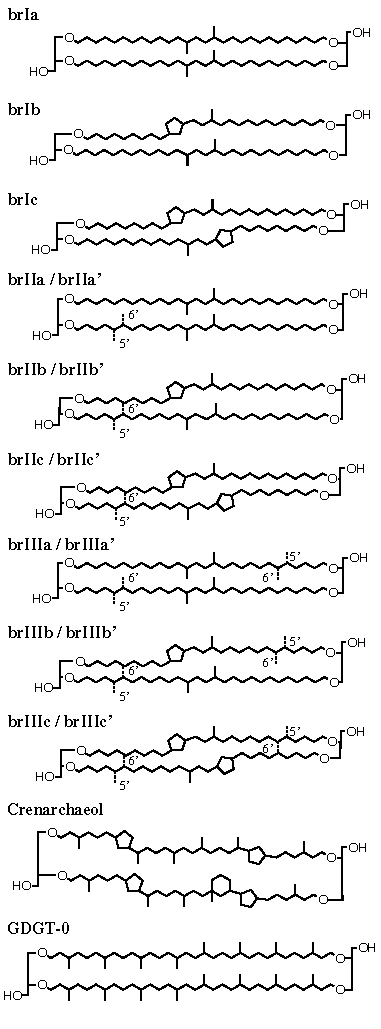
\includegraphics[]{Thesis_Figures/Ch5FigS1}}
	\caption[Core lipid GDGT structures]{Core lipid GDGT structures showing both 5-methyl and 6-methyl homologues for branched compounds.}
	\label{Ch5Fig:S1} 
\end{figure}

% Reset figure style for subsequent chapters
\renewcommand\thefigure{\thechapter.\arabic{figure}}
